%%%%%%%%%%%%%%%%%%%%%%%%%%%%%%%%%%%%%%%%%%%%%%%%%%%%%%%%%%%%%%%%%%%%%%
%%                Informações sobre o Autor e Distribuição          %%
%%%%%%%%%%%%%%%%%%%%%%%%%%%%%%%%%%%%%%%%%%%%%%%%%%%%%%%%%%%%%%%%%%%%%%

% Template Desenvolvido por: 
% Maurício Fernandes de Oliveira Assis
% Gerente de Projetos da Power Jr.
%
% Objetivo:
% Este template foi criado para a Power Jr. com o propósito de padronizar 
% a elaboração de memoriais descritivos, garantindo clareza, organização e 
% profissionalismo na apresentação de projetos de climatização e outras 
% áreas de engenharia.

% Estrutura do Template:
% - Arquivo `corpo.tex`:
%   Este arquivo é destinado à construção do conteúdo principal do memorial 
%   descritivo. É nele que as informações específicas de cada projeto devem 
%   ser inseridas, como descrição, especificações técnicas e outros detalhes 
%   relevantes.
% 
% - Arquivo `lib/power.sty`:
%   Este arquivo contém as configurações de formatação do documento, incluindo:
%   estilos de texto, estrutura das seções, sumário e outras configurações. 
%   Alterações podem ser realizadas neste arquivo para adaptar o template 
%   às necessidades específicas de cada projeto.

% Dados de Contato da Empresa:
% Empresa: Power Jr.
% Endereço: Av. Manoel Novais, 1064, Centro, CEP: 47600-000, Bom Jesus da Lapa, BA
% Email: empresa.powerjr@gmail.com

% Informações Adicionais:
% - Data de criação do template: 18/11/2024
% - Repositório GitHub para contribuições e atualizações:
%   https://github.com/mauriciofernandes123
%%%%%%%%%%%%%%%%%%%%%%%%%%%%%%%%%%%%%%%%%%%%%%%%%%%%%%%%%%%%%%%%%%%%%%

\textit{Aviso: Todos os dados abaixo são fictícios, elaborados apenas para demonstração do formato de um Memorial Descritivo para a Power Jr.}

\section{Apresentação Geral}

Nesta seção deve-se colocar uma breve apresentação do projeto.
 

\section{Objetivos}

Deve-se adicionar os objetivos do memorial descritivo de forma detalhada.

\section{Normas Técnicas Aplicadas}
Exemplo:

O projeto foi desenvolvido em conformidade com as seguintes normas da ABNT:
\begin{itemize}
    \item NBR 5410 – Instalações Elétricas de Baixa Tensão;
    \item NBR 15575 – Edificações Habitacionais: Desempenho;
    \item NBR 6120 – Cargas para o Cálculo de Estruturas de Edificações.
\end{itemize}

\section{Relação de Desenhos do Projeto}
Os desenhos técnicos disponíveis incluem:
\begin{itemize}
    \item Planta baixa;
    \item Cortes e fachadas;

\end{itemize}

\section{Base de Cálculo e Carga Térmica}
\subsection{Parâmetros Gerais}
Para o cálculo da carga térmica, foram considerados os seguintes parâmetros:
\begin{itemize}
    \item Temperatura externa: 30°C;
    \item Temperatura interna: 22°C;
    \item Ocupação: 4 pessoas.
\end{itemize}

\subsection{Resultado de Cálculo dos Ambientes}
A carga térmica total estimada para os ambientes é de 24.000 BTU/h.

\section{Descrição dos Equipamentos}
\subsection{Fan Coil}
\subsubsection{Unidade Básica}
Modelo: FCU-250. Potência de 2,5 TR.

\subsubsection{Ventilador}
Ventilador centrífugo com motor trifásico.

\subsubsection{Trocadores de Calor}
Trocador de calor aletado com tubos de cobre e aletas de alumínio.


\subsubsection{Exemplo de figura}

\begin{figure}[h]
    \centering
    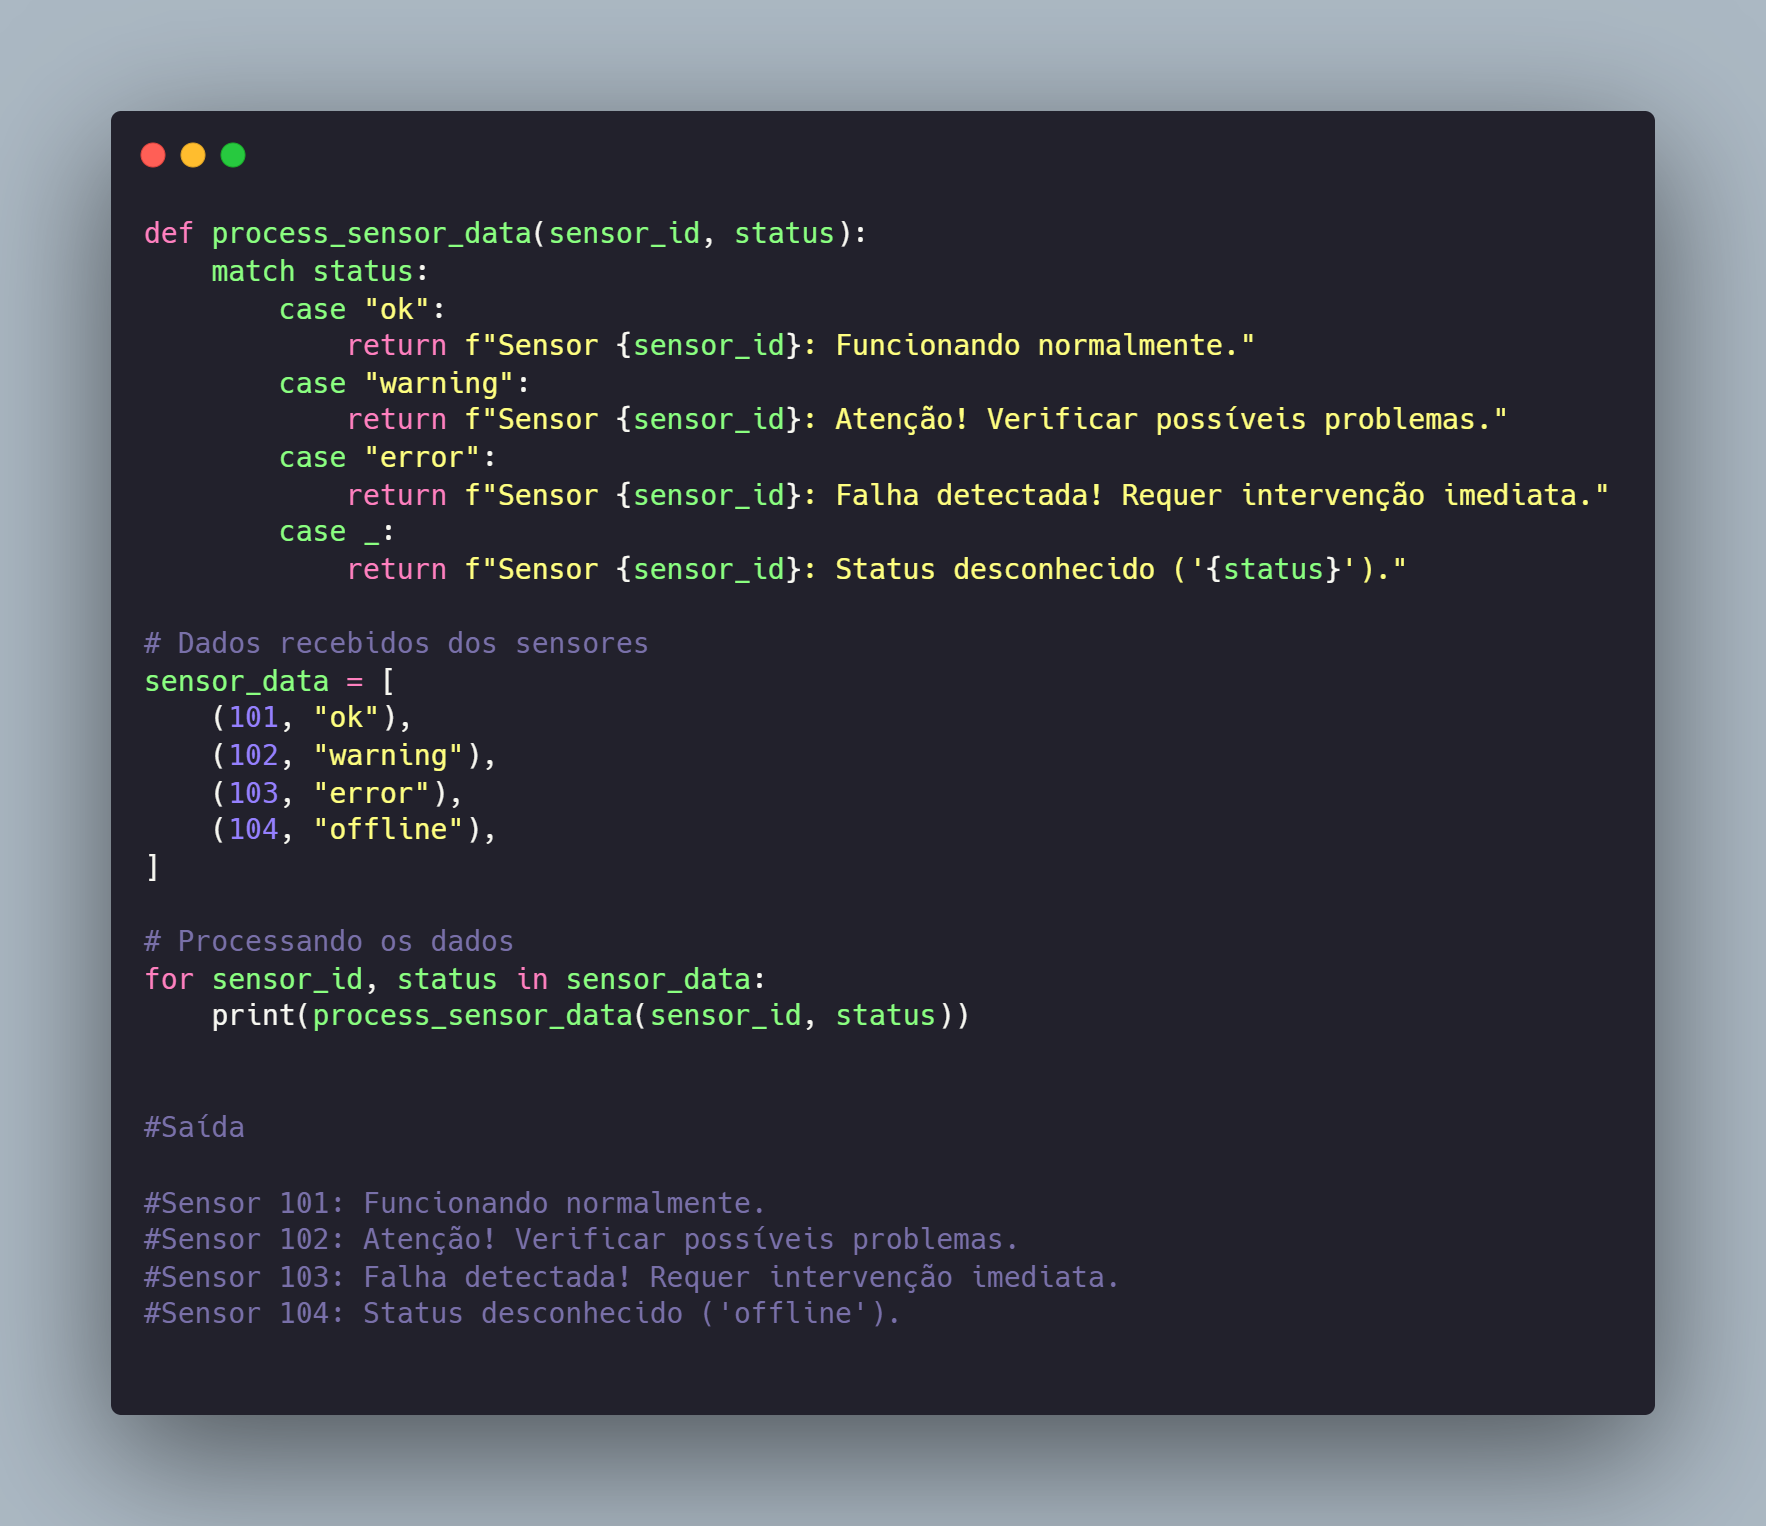
\includegraphics[width=12cm]{Figuras/carbon.png}
    \caption{Exemplo de Figura}
    \label{fig:exemplo_equipamento}
    \vskip 1mm
    \textbf{Fonte:} Power Jr. (2024).
\end{figure}

\subsection{Dutos de Distribuição de Ar}
\subsubsection{Construção}
Dutos de chapa galvanizada conforme norma SMACNA.

\subsubsection{Isolamento Térmico}
Isolamento com lã de vidro de 25 mm.

\section{Etapas da Construção}
\subsection{Terraplanagem}
Realizada para garantir a estabilidade do terreno.

\subsection{Alvenaria}
Paredes externas construídas com blocos cerâmicos de 15 cm.

\subsection{Acabamento}
Revestimento em porcelanato nas áreas molhadas e laminado nas áreas internas.

\section{Exemplo de tabela}
\begin{table}[h!]
\centering
\begin{tabular}{ccc}
\toprule
\textbf{Etapa} & \textbf{Duração (meses)} & \textbf{Responsável} \\ \midrule
Terraplanagem & 1 & Equipe de Terraplanagem \\ 
Fundação & 2 & Engenheiro Civil \\ 
Estrutura & 3 & Engenheiro Civil \\ 
Acabamentos & 6 & Construtora \\ 
Paisagismo & 1 & Arquiteto \\ \bottomrule
\end{tabular}
\caption{Exemplo de Tabela}
\label{tab:cronograma}
\end{table}

\section{Instalações}

Todas as instalações elétricas deverão obedecer, integralmente, às disposições da norma NBR5410 da ABNT (Associação Brasileira de Normas Técnicas) e as orientações do presente documento. A alimentação elétrica disponível para os sistemas é trifásica 220V / 60Hz.